\chapter{Testing} \label{ch:testing}
\todo{Write section \texttt{testing}}
Testing video games is not an easy process.
This task is very different from testing other software.
In other software the most important thing is the functionality, however in games the visuals are just as important.
That means that testing if for example the player model was rendered is not enough, it also has to be tested if it was rendered correctly.
That is made even more difficult by the fact that the game uses the GPU to render the graphics.
All these difficulties make testing in code very difficult, which is why apart from unit testing we focused on manual testing.
\todo{Add source that says how video games are usually tested}

\section{Unit testing} \label{sec:unit_testing}
Unit testing was used to test particular methods and classes.
These tests check if the methods behave as expected.
However, even using mocking frameworks some things, in particular things connected to the graphics, cannot be unit tested.
Because of that the most important part of testing was manual testing described in \autoref{sec:manual_testing}.
\section{Manual testing} \label{sec:manual_testing}
Manual testing is responsible for testing the game as a whole.
It tests the results and not particular methods or parts of the code.
Manual tests scenarios were created that describe in detail what should happen in the game after some actions are performed.
These tests cover the entirety of the application and can be viewed at \url{https://github.com/Non-Euclidean-World/HyperTesting}.
The tests are written as Markdown files that have references to image and video files that show the expected behavior of the game.
The test cases are divided into four parts:
\begin{enumerate}
  \item Title - The name of the test case.
  \item Description - What the test case is supposed to test.
  \item Prerequisites - What has to be done before the test case can be performed.
  \item Steps - A table that describes the actions that have to be performed and their expected results.
\end{enumerate}

Below is an example of a test case.
It is important to note that the test case has been modified to fit the paper format by changing links to the images into references.

\todo{Might want to write a specific test case to put here since all the nice ones have videos in them}

\begin{mdframed}[backgroundcolor=gray!20]
  \subsection*{Flashlight works}\label{flashlight-works}

  \subsubsection*{Description}\label{description}

  Test case for checking if the player can use the flashlight. The test
  case should work for all geometries.

  \subsubsection*{Prerequisites}\label{prerequisites}

  The game is running.

  The camera is in 1st person mode.

  \subsubsection*{Steps}\label{steps}

  \begin{longtable}[]{@{}
    >{\raggedright\arraybackslash}p{(\columnwidth - 4\tabcolsep) * \real{0.3333}}
    >{\raggedright\arraybackslash}p{(\columnwidth - 4\tabcolsep) * \real{0.3333}}
    >{\raggedright\arraybackslash}p{(\columnwidth - 4\tabcolsep) * \real{0.3333}}@{}}
    \toprule\noalign{}
    \begin{minipage}[b]{\linewidth}\raggedright
      Step
    \end{minipage} & \begin{minipage}[b]{\linewidth}\raggedright
                       Action
                     \end{minipage} & \begin{minipage}[b]{\linewidth}\raggedright
                                        Expected Result
                                      \end{minipage}                                                   \\
    \midrule\noalign{}
    \endhead
    \bottomrule\noalign{}
    \endlastfoot
    1                                           & Press \texttt{Y}                            & The flashlight should turn on, see
    here. (\autoref{fig:flashlight_on})                                                                                            \\
    2                                           & Press \texttt{Y} again                      & The flashlight should turn off     \\
  \end{longtable}

  \begin{figure}[H]
    \centering
    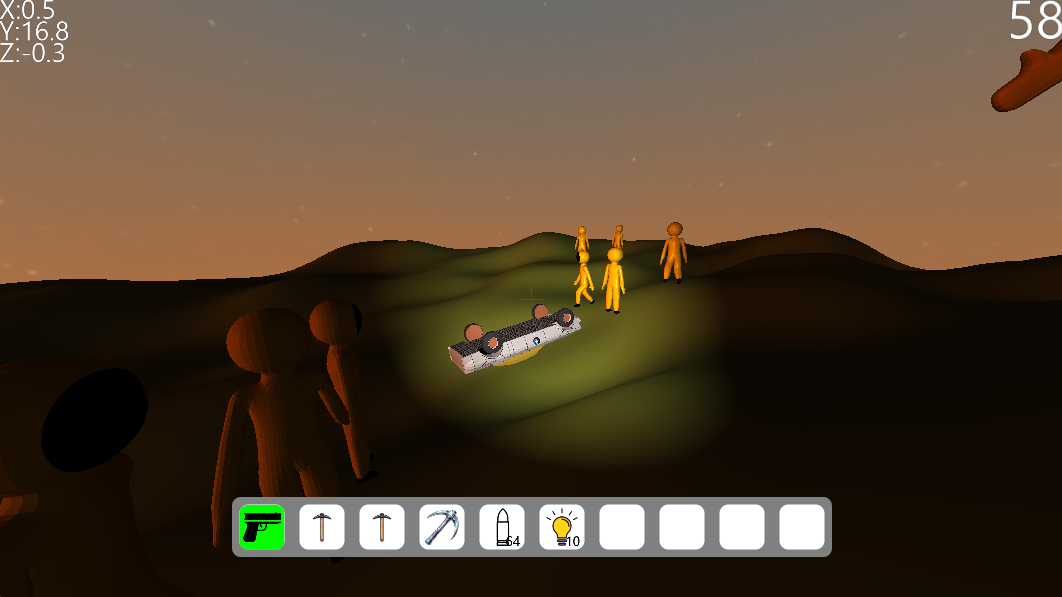
\includegraphics[width=0.5\textwidth]{chapters/tests/resources/flashlight.png}
    \caption{The flashlight is on.}
    \label{fig:flashlight_on}
  \end{figure}
\end{mdframed}
